% !TeX root = ../main.tex
\chapter{Detailed State Machines}
\label{appendix:state-machines}

The business state machine of the Document and Video Pipeline is
already presented in Chapter~\ref{chap:phan-tich-thiet-ke} because it
governs the user-visible processing status. The two state machines
below cover separate concerns -- broker-level retry semantics and
the per-card content review lifecycle -- and are placed here so they
do not interrupt the main design narrative.

\section{Asynchronous Job State (BullMQ)}
\label{appendix:state-async-job}

Broker jobs in BullMQ have a state machine that is intentionally
\emph{independent} from business state. Job-level retries do not move
a document/video out of its current business state; conversely, a
finished job does not by itself promote a business aggregate.

\begin{figure}[H]
    \centering
    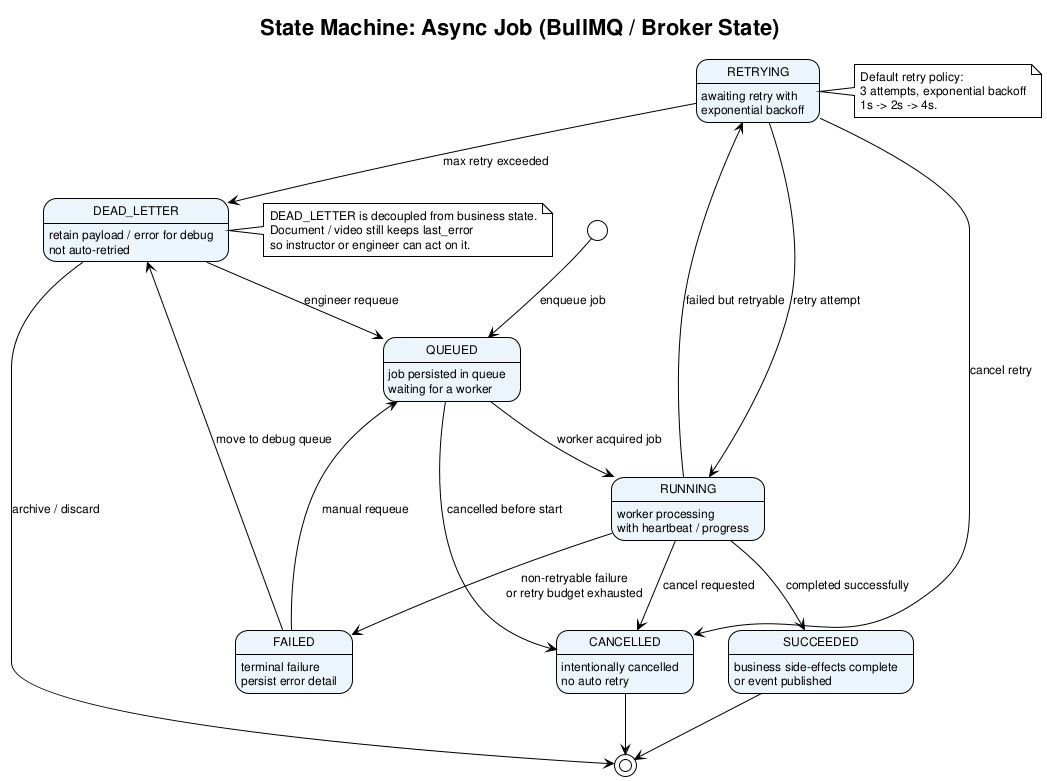
\includegraphics[width=0.9\textwidth,height=0.72\textheight,keepaspectratio]{diagrams/state_machine_async_job.png}
    \caption{State machine of asynchronous jobs in the broker.}
    \label{fig:state-machine-async-job}
\end{figure}

\textbf{Retry policy.} Three attempts with exponential backoff
($1\text{s} \to 2\text{s} \to 4\text{s}$). After the maximum retries,
the job moves to \texttt{DEAD\_LETTER} for manual debugging. Engineers
can requeue it from the BullMQ dashboard.

\section{Content Review State (LessonCard / QuizItem)}
\label{appendix:state-content-review}

Generated artifacts go through an explicit Human-in-the-Loop review
lifecycle before being visible to learners.

\begin{figure}[H]
    \centering
    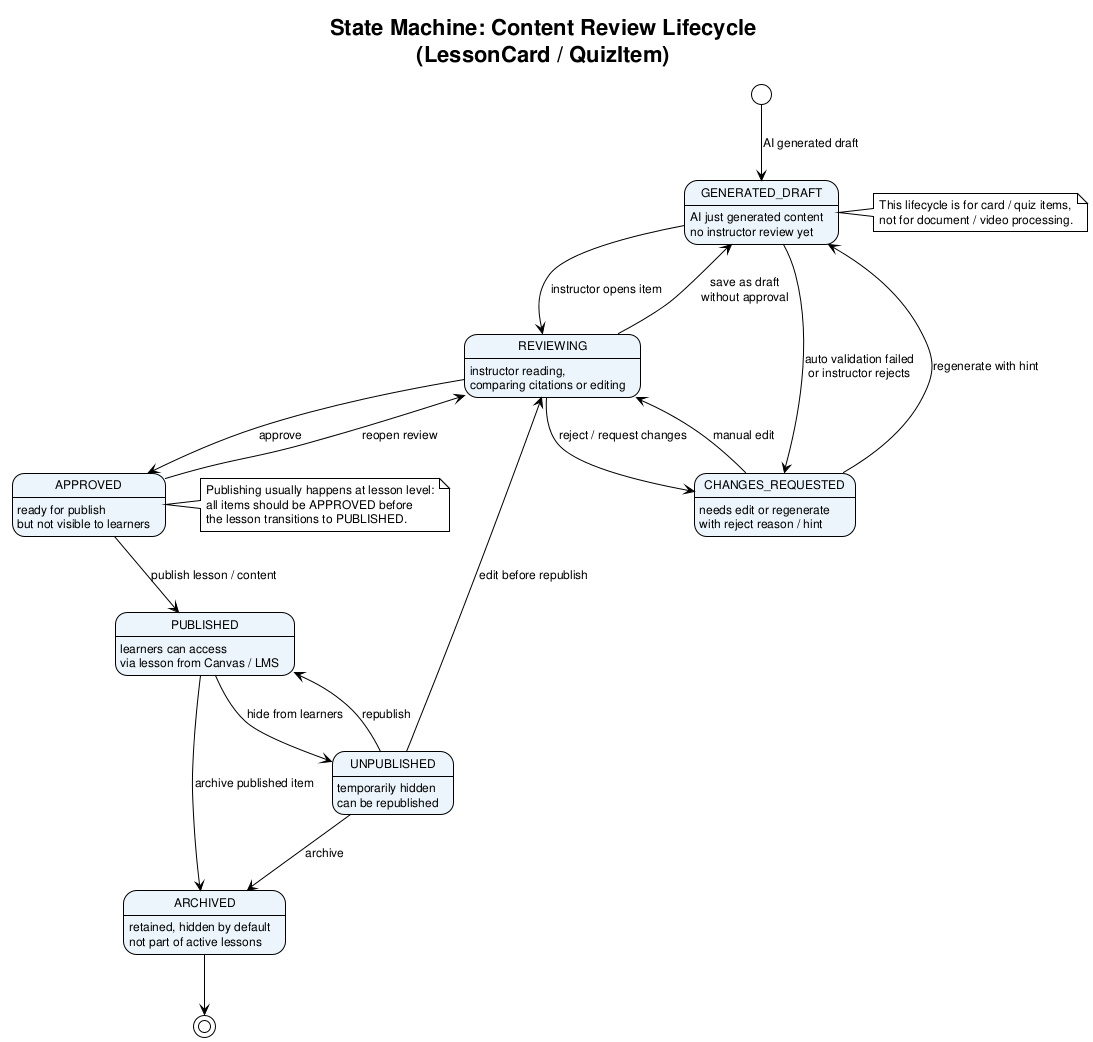
\includegraphics[width=0.9\textwidth,height=0.72\textheight,keepaspectratio]{diagrams/state_machine_content_review.png}
    \caption{Review lifecycle state machine for cards and quizzes.}
    \label{fig:state-machine-content-review}
\end{figure}

\begin{table}[H]
    \centering
    \caption{Review states of generated content.}
    \label{tab:review-states-appendix}
    \begin{tabular}{|p{4cm}|p{9.5cm}|}
        \hline
        \textbf{State} & \textbf{Meaning} \\
        \hline
        \texttt{GENERATED\_\allowbreak DRAFT}
            & AI generated it; no one has reviewed it yet. \\
        \hline
        \texttt{REVIEWING}
            & Instructor is reviewing/editing. \\
        \hline
        \texttt{CHANGES\_\allowbreak REQUESTED}
            & Instructor rejected it and requested regeneration or edit. \\
        \hline
        \texttt{APPROVED}
            & Approved and ready to publish. \\
        \hline
        \texttt{PUBLISHED}
            & Learners can access it. \\
        \hline
        \texttt{UNPUBLISHED}
            & Hidden from learners; instructor may republish. \\
        \hline
        \texttt{ARCHIVED}
            & Stored for history; not shown by default. \\
        \hline
    \end{tabular}
\end{table}
